
%%%%%%%%%%%%%%%%%%%%%%%%%%%%%%%%%%%%%%%%%%%%%%%%%%%%%%%%%%%%%%%%%%%%%%%%%%%%%%%%
% Tikz Intro:

\usetikzlibrary{shapes,arrows,graphs}

\tikzstyle{statement}  = [rectangle, draw, rounded corners, fill=blue!20, text centered, very thick, minimum size=1cm]
\tikzstyle{expression} = [rectangle, draw, rounded corners, fill=red!20,  text centered, very thick, minimum size=1cm]

%%%%%%%%%%%%%%%%%%%%%%%%%%%%%%%%%%%%%%%%%%%%%%%%%%%%%%%%%%%%%%%%%%%%%%%%%%%%%%%%

% Gode opgaver:
%    https://adriann.github.io/programming_problems.html

	\todo{Hvordan skriver vi til deltagerne? Skriver vi \emph{I}? Undgår vi at rette os mod dem?}
\chapter{Kontrol og Metoder}

	\todo{@Beatrice: Kan du ikke tage for-each løkker? Måske som ekstra?}

    I sidste kapitel blev variabler, aritmetiske udtryk og
    \emph{if-statements} introduceret. Med disse dele kan man lave det
    der heder et \emph{straight-line program}, også kendt som kedelige
    programmer. Vi er ofte stillede over for opgaver som ikke kan
    løses ekslusivt med sådanne programmer. Vi behøver mere
    udtrykskraft, end hvad aritmetik og basal beslutningsevner kan
    give os.

    For eksempel vil vi gerne kunne sige ting som ``gør \emph{det her} indtil
	\emph{dette} sker'' eller ``gør \emph{dette}, først for \emph{1}, og så for
	\emph{2}, osv.''

	Af denne grund indeholder mange programmerings-sprog, inklusiv Java,
	mekanismer for at kunne udtrykke sådanne problemer, og det er disse
	mekanismer vi vil dække i dette kapitel.

	Det er vigtigt at tage i mende at programmører er dåvne dyr, og vil gerne
	udtrykke sig selv nemt. Derfor har Java rigtig mange mekanismer som teknisk
	set kan gøre det samme, men som er mere bekvemme i visse situationer.

    Dette kapitel vil dække mange af disse mekanismer. Du behøver ikke
    lære dem alle med de samme. Selv de bedste programmører glemmer
    hvordan man skriver nogle af disse. Følgende overordnet emner er
    dækket i dette kapitel:

	\begin{itemize} % Denne udgiver har også følgende selvhjælps-bøger på markedet:
		\item Løkker: Sådan får du mere kontrol
		\item Funktioner: Forbedre dine metoder
		\item Arrays: Få styr på dine variabler.
	\end{itemize}

\section{Løkker}

    En klassisk problemstilling er at gøre gentage noget kode en hvis
    mængden af gange. Der er mange løsninger, hvoraf løkker er en af
    de simpleste. I denne sektion dækker vi simple løkker og kigger
    lidt på nogle mere advanceret måder at bruge løkker på.

	\subsection{While-løkker}

        \JavaInline{while} er den simpleste type af løkke. Dette er ligesom at
		sige: ``Mens at A gælder, sørg for at gøre B.'' For eksempel:

		``Mens at gulvet er beskidt, bør du feje gulvet.''

		Dette er i modsætning til \JavaInline{if}-udstryk, hvor der udtrykkes
		``Hvis A gælder, gør B èn enkelt gang.''

		Anatomien af en \JavaInline{while}-udstryk er meget lig det af et
		\JavaInline{if}-udstryk, du skifter bare \JavaInline{if} ud med
		\JavaInline{while}, som kan ses i \autoref{lst:while-example-1}.

		\begin{JavaCode}{Et eksempel på en \texttt{while}-løkke}{lst:while-example-1}
			while (betingelse) {
				krop;
			}
		\end{JavaCode}

        Man kalder koden mellem paranteserne for while-udtrykkets
        ``betingelse'', koden mellem tuborg-klammerne for ``kroppen''.
        Her gennemgang af kroppen er en ``'iteration'.  Første gang
        løkken ses, kigges der på betingelsen, og hvis denne er
        \emph{sand} så køres kroppen, ellers hopper man over og
        fortsætter uden at køre løkken. Hvis man til gengæld har kørt
        kroppen, enten første gang eller efterfølgende, og er nået
        enden, så spørger man igen om betingelsen er \emph{sand}, hvis
        ja, køres kroppen igen, hvis ikke, fortsætter vi efter løkken.
        Denne process er illustreret i
        \autoref{fig:while-loop-illustrated}. Et eksempel på en
        løkke kan findes i \autoref{lst:while-example-3}.

        % Følgende er baseret på:
        %    https://upload.wikimedia.org/wikipedia/commons/4/43/While-loop-diagram.svg

        \begin{figure}
        \center
        \tikzstyle{flow} = [draw, very thick, rounded corners]
        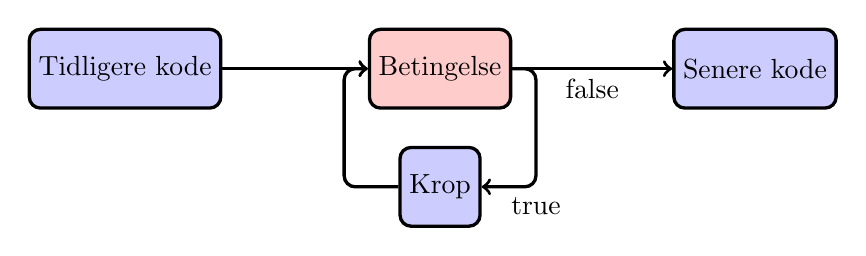
\begin{tikzpicture}[node distance = 4cm, auto]
            \node[statement] (previous) {Tidligere kode};
            \node[expression, right of=previous] (condition) {Betingelse};
            \node[statement, below of=condition, node distance=1.5cm] (body) {Krop};
            \node[statement, right of=condition] (after) {Senere kode};

            \path [flow, ->] (previous.east) -- (condition.west);
            \path [flow, ->] (condition.east) -- node[auto, swap] {false} (after.west);
            \path [flow, <-] (condition.west) -- +(left:3mm) |- (body.west) ;
            \path [flow, ->] (condition.east) -- +(right:3mm) |- node {true} (body.east);
        \end{tikzpicture}
        \caption{While-løkker}
        \label{fig:while-loop-illustrated}
        \end{figure}

		\begin{JavaCode}{Et program der næsten kun består af en while-løkke. Den gennemgår 10 iterationer, før den stopper. Læg mærke til at n er alle tal op til 10, på forskellige tidspunkter.}{lst:while-example-3}
			int n = 1;
			while (n <= 10) {
				System.out.println(n + " linjer af ligegyldig data.");
				n++;
			}
		\end{JavaCode}

        \autoref{lst:while-example-3} stopper efter 10
        iterationer, men det er muligt at lave while-løkker der aldrig
        stopper.  Det er faktisk så nemt at de fleste, ved uheld,
        kommer til at lave en nu og da. Se
        \autoref{lst:while-hello-forever} for et program som
        gentagende skriver ``hej''. Det er selvfølgelig ikke så
        brugbart et program, men det viser en problematik: Hvad gør vi
        hvis vores program aldrig stopper? I har sikkert oplevet et
        program der stoppede med at reagere, og var nød til at blive
        ``drabt'', for at I kunne fortsætte. Det er præcis det samme
        med jeres egne programmer, hvis de indeholder uendelige
        løkker. \footnote{Et relateret spørgsmåle er ``kan man lave et
        program som siger om et program stopper eller ej?''. Det er
        muligt at lave et program, som svarer for \emph{nogle}
        programmer, men umuligt at lave en som kan svare for
        \emph{alle} programmer.  (Læg mærke til at programmet skulle
        svare om det selv stoppede.) Denne problematik kaldes for
        \emph{The Halting Problem}, og blev bevist af \emph{Allan
        Turing} i 1936.}

		\begin{JavaCode}{Et program der aldrig ender.}{lst:while-hello-forever}
			System.out.println("Hello World!");
			while (true) {
				System.out.println("Hello again!");
			}
		\end{JavaCode}

        Det giver sjældent mening at have sådanne uendelige
        løkker\footnote{De fleste programmer du kører på din computer
        eller smartphone har uendelige løkker, gemt dybt i koden, da
        disse programmer skal køre indtil brugeren lukker dem.}, og de
        fleste løkkers betingelser blive \emph{falsk} på et
        tidspunkt.

		\begin{exercise}
			Copenhagen Suborbitals har kontaktet dig, for at lave en maskine til
            at tæller ned fra 10, og vise "Affyring!", i stedet for 0.
            Tag gerne inspiration fra
            \autoref{lst:while-example-3}.
		\end{exercise}

		\begin{exercise}
            Brug en \JavaInline{while}-løkke til at summerer tallene
            fra 1 til 100, og derefter viser det på skærmen.
		\end{exercise}

		\begin{exercise}
            Skriv et program som tæller op fra \(1\) til \(100\), og
            for hvert tal, vis tallet, og hvis det kan deles af 3 vis
            ``foo'', og hvis det kan deles af 5 vis ``bar''. Hvis det
            deles af både 3 og 5, vis ``foobar''.  I får brug for et
            \JavaInline{if}-udtryk.
        \end{exercise}

		\begin{exercise}
            Brug en \JavaInline{while}-løkke til at summerer tallene
            fra 1 til 100, men ignorer tal der ikke deles af 3 eller
            5. Så \(1, 2, 4, 7, 8, \dots\) skal ikke inkluderes, mens
            at \(3, 5, 6, 9, 10, 12, \dots\) skal.
        \end{exercise}

	\subsection{For-løkker}

		I sidste sektion så vi kan tælle op med et \JavaInline{while}-udtryk.
        De fleste programmører syntes ikke det er en god måde at tælle
        på, da \JavaInline{n} defineres, sammenlignes og opdateres på
        helt forskellige steder i koden.  Det kan blive svært at holde
        styr på i store programmer, hvilket er hvorfor Java har
        \JavaInline{for}-løkken, som samler den information i
		èt sted.

		\begin{JavaCode}{Et eksempel på en \texttt{for}-løkke}{lst:for-example-1}
			for (definition; betingelse; opdatering) {
				krop;
			}
		\end{JavaCode}

        \begin{figure}
        \center
        \tikzstyle{flow} = [draw, very thick, rounded corners]
        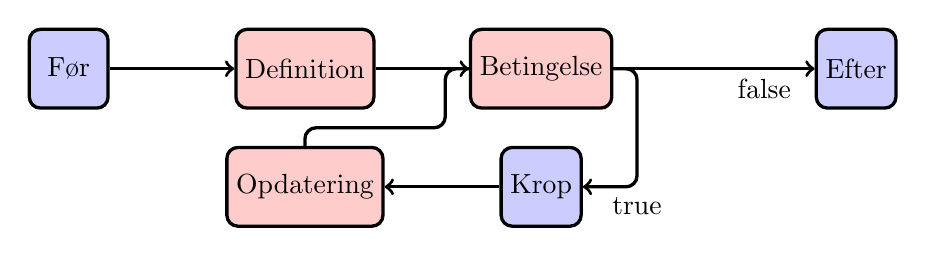
\begin{tikzpicture}[node distance = 3cm, auto]
            \node[statement] (previous) {Før};
            \node[expression, right of=previous]   (definition) {Definition};
            \node[expression, right of=definition] (condition)  {Betingelse};
            \node[expression, below of=definition, node distance=1.5cm]  (update)     {Opdatering};
            \node[statement, below of=condition, node distance=1.5cm] (body) {Krop};
            \node[statement, right of=condition, node distance=4cm] (after) {Efter};
            \coordinate[below right of=definition, node distance=1.061cm] (updtocond);

            \path [flow, ->] (previous.east)   -- (definition.west);
            \path [flow, ->] (definition.east) -- (condition.west);
            \path [flow, ->] (condition.east) -- node[auto, swap, near end] {false} (after.west);
            \path [flow, ->] (condition.east) -- +(right:3mm) |- node {true} (body.east);
            \path [flow, ->] (body.west) -- (update.east);
            \path [flow] (condition.west) -- +(left:3mm) |- (updtocond) -| (update.north);
        \end{tikzpicture}
        \caption{For-løkker}
        \label{fig:for-loop-illustrated}
        \end{figure}

		Strukturen af for-løkker er ret involveret, men det hjælper at
		sammenligne med \JavaInline{while}-udstryk, og se hvordan at forskellige
		dele af koden som tidligere var sprædt, nu er samlet.

        For-løkker inkluderer ``definitioner'', ``betingelse'',
        ``krop'' og ``opdatering''. Når en for-løkke først ses, vil
        definitionen køres. Denne sætter ofte en variable til en
        bestem værdi. Derefter testes betingelsen som i while-løkker.
        Hvis denne er \emph{sand}, køres kroppen. Når kroppen er
        færdi, køres opdateringen. Denne sætte værdien af variablen
        til hvad den skal være i den næste iteration.

		\begin{JavaCode}{Et ``brugbart'' for program. Sammenlign med \autoref{lst:while-example-3}.}{lst:for-example-1}
			for (int n = 1; n <= 10; n++) {
				do-System.out.println(n + " linjer af ligegyldig data.");
			}
		\end{JavaCode}

        For-løkker er bare en anderledes måde at skrive while-løkker
        på, hvor al informationen som løkken anvender, samles i et
        sted, og gør det derfor nemmere at læse koden.

		\begin{exercise}
            Brug en \JavaInline{for}-løkke til at summerer tallene
            fra 1 til 100, men ignorer tal der ikke deles af 3 eller
            5. Overvej forskellen mellem \JavaInline{while} versionen
            fra sidste afsnit, og denne version.
        \end{exercise}

		\begin{exercise}
			Det er ofte fortalt hvordan at Gauss i sine unge dage, forpurrerede sin
			lærers plan om at få ham til at tie stille. Hun bedte ham lægge tallene
			fra \(1\) til \(100\) sammen, i håbet at dette ville optage det unge
			geni i lidt tid. Gauss realiserede dog at der måtte være en bedre måde
			at løse problemet på, og udledte formularen \(\frac{n\cdot(n+1)}{2}\).
			Han svarede hurtigt \(5050\), og så måtte læreren finde på en anden
			kedelig opgave.

			Brug et \emph{for-løkke} til at beregne \(1^2+2^2+\dots+100^2\).
		\end{exercise}

		\begin{exercise}
			Der er selvfølgelig ikke noget som forhindrer at du bruger et
			\emph{for-løkke} ind i et andet \emph{for-løkke}, og dette kan nogle gang
			være vældig praktisk.

			\todo{Find på opgave!}
		\end{exercise}

	\subsection{Break-udtryk}

		Sommetider vil man gerne gå ud af en løkke tidligt. Dette tillader
        \JavaInline{break}-keywordet os at gøre. Når koden rammer en
        \JavaInline{break}, vil den straks hoppe ud af den
        \emph{inderste} løkke.

        \begin{JavaCode}{Et brugbart while program som stopper efter 10 linjer, på trods af at betingelsen aldrig bliver \emph{falsk}.}{lst:break-example-1}
			int n = 1;
			while (true) {
				System.out.println(n + " linjer af ligegyldig data.");
				n++;
				if (n == 10)  break;
			}
		\end{JavaCode}

        Læg mærke til at \autoref{lst:break-example-1},
        \autoref{lst:for-example-1} og \autoref{lst:while-example-3}, alle
        sammen gør præcis det samme når de køres, selvom de ser
        anderledes ud. Dette illustrerer hvordan der altid er flere
        måder at gøre ting på.

        \todo{Tilføj en opgave, som viser at man godt kan klare sig
        uden break, men at break er pænere.}

	\subsection{Do ... while}

        While-løkker tjekker betingelsen før hver iteration, men nogle
        gang vil vi gerne tjekke betingelsen, efter vi har kørt
        iterationen. For eksempel kunne vi lave en beregning, og
        baseret på den beslutte om vi ville videre. Dette løser
        \emph{do-while} udtryk på en pæn måde. Sammenlign
        \autoref{lst:dowhile-example-1} og
        \autoref{lst:dowhile-example-2}. Se \autoref{fig:do-while-loop-illustrated}.

		\begin{JavaCode}{Vil aldrig skrive ``Hej med dig''.}{lst:dowhile-example-1}
			while (false) {
				System.out.println("Hej med dig");
			}
		\end{JavaCode}

		\begin{JavaCode}{Vil skrive ``Hej med dig'' en enkelt gang.}{lst:dowhile-example-2}
			do {
				System.out.println("Hej med dig");
			} while (false)
		\end{JavaCode}

        \begin{figure}
        \center
        \tikzstyle{flow} = [draw, very thick, rounded corners]
        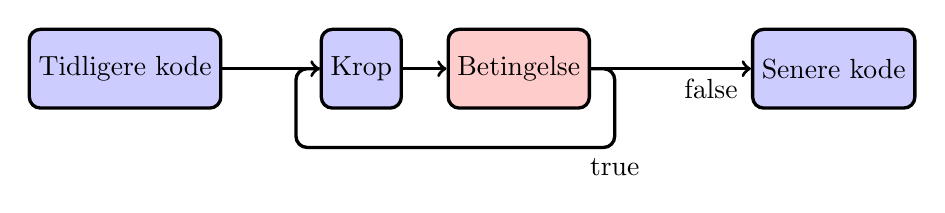
\begin{tikzpicture}[node distance = 3cm, auto]
            \node[statement] (previous) {Tidligere kode};
            \node[statement, right of=previous] (body) {Krop};
            \node[expression, right of=body, node distance=2cm] (condition) {Betingelse};
            \node[statement, right of=condition, node distance=4cm] (after) {Senere kode};
            \coordinate[below of=condition, node distance=1cm] (loop);

            \path [flow, ->] (previous.east)  -- (body.west);
            \path [flow, ->] (body.east)      -- (condition.west);
            \path [flow, ->] (condition.east) -- node[auto, swap, near end] {false} (after.west);
            \path [flow]     (condition.east) -- +(right:3mm) |- node {true} (loop);
            \path [flow]     (body.west)      -- +(left:3mm)  |- (loop);
        \end{tikzpicture}
        \caption{Do-while-løkker}
        \label{fig:do-while-loop-illustrated}
        \end{figure}

		For eksempel:

		\begin{JavaCode}{Konstruerer en streng som måler længen af sig selv i de forskellige iterationer.}{lst:dowhile-example-3}
			String a = "";
			do {
				a = " " + a.length();
			} while (a.length <= 10);
			System.out.println(a);
		\end{JavaCode}

        I gamle dage var \JavaInline{do ... while} mere populært end
        \JavaInline{while}, da \JavaInline{do ... while} var
        hurtigere, idé at den ikke behøver at tjekke om betingelsen er
        sand, før første iteration.

	\subsection{Continue}

        Ligesom man ind i mellem gerne vil hoppe ud af en løkke, vil
        vi ind i mellem gerne oppe over en specifik iteration. Dette
        gøres med \JavaInline{continue}-keyword.

        \begin{JavaCode}{Kode der anvender \texttt{continue} til at kun vise de lige tal. Læg mærke til at derp giver resten a divideret med b, også kaldt \texttt{modulo}.}{lst:unknown-a}
			for (int i = 1; i <= 10; i++) {
				if (i \% 2 == 0)  continue;
				System.out.println(i);
			}
		\end{JavaCode}

        \todo{Tilføj en opgave, som viser at man godt kan klare sig
        uden continue, men at continue er pænere.}

\section{Funktioner}

    Sidste kapitel introducerede \emph{funktioner}\footnote{Også
    kaldet \emph{metoder} eller \emph{procedurer}.} som sorte-bokse,
    der gør arbejde for dig. For eksempel \JavaInline{Math.abs} som
    giver den absolutte værdi af hvadend den bliver givet. I denne
    sektion viser vi hvordan man laver sine egne funktioner, en
    færdighed som viser sig at være meget brugbar.

    Vi kalder hvad en funktion giver tilbage for dens
    \emph{retur-værdi} eller hvad funktionen \emph{returnerer}. Vi
    kalder hvad vi giver den, dvs. det som sættes mellem paranteser,
    for funktionens \emph{argumenter}.

    \todo{@Beatrice: Husk at forklare \texttt{private} og \texttt{public}.}

	\subsection{En funktions udseende}

		I har allerede set en funktion, nemlig \JavaInline{main}-funktionen, hvor i
		indtil videre har skrevet alle jeres programmer i:

		\begin{JavaCode}{Main funktion}{lst:main-function}
			public static void main(String[] args) {
				// Ting her...
			}
		\end{JavaCode}

		En funktion består af dens \emph{signatur} og dens \emph{krop}.

        Dens signatur er \JavaInline{public static void main(String[] args)}
        delen.  Dette fortælles os lidt om funktionen: dens
        navn \JavaInline{main}; dens retur-værdi \JavaInline{void} (ingenting); og
        dens argumenter \JavaInline{String[] args}, hvilket er en liste af
        strenge, som funktionen kalder \JavaInline{args}.  Signaturen for
        \JavaInline{main} siger også at den er \JavaInline{static} og
        \JavaInline{public}. Disse egenskaber kan ignoreres for nu, da de
        først bliver relevant når man kender til klasser.

        En funktions krop er \JavaInline{// Ting her...} delen. Alt
        mellem krølleparanteserne er funktionens krop, og beskriver
        hvad funktionen gør.  Hvis funktionen har en retur-type, skal
        \JavaInline{return}-keywordet opstå mindst én gang i kroppen.
        \JavaInline{return} er hvordan man går ud af en funktion,
        samtidig med at give en retur-værdi.  \JavaInline{return} kan
        ses som en \JavaInline{break} for funktioner.
        \JavaInline{main} funktionen ovenover behøver ikke en
        \JavaInline{return}, men \autoref{lst:guarenteed-random}
        skal have en, da den har en retur-type.

		\begin{JavaCode}{xkcd 221}{lst:guarenteed-random}
			public int getRandomNumber() {
				return 4;  // chosen by fair dice roll.
			}
		\end{JavaCode}

        Signaturen er hvordan man skal snakke med funktionen, og
        kroppen er hvad den egentlig gør. Læg mærke til at hvis
        funktionen ikke skal have en retur-værdi, skal den gives
        retur-typen \JavaInline{void}, hvilket står for ``jeg har ingen retur-type''.

	\subsection{Eksempel funktion: fakultet}

        Hvis vi skulle skrive \emph{faktoriel}-funktionen som en
        funktion i Java, ville vi først spørge os selv: ``hvad
        returnerer faktoriel og hvad er dens argumenter?'' Det virker
        måske trivielt, i dette eksempel, men stadig et vigtigt
        spørgsmål. Derefter skal vi spørge: ``Men hvad er det den
        gør?''

        Faktoriellen er defineret som \(a! = a \cdot (a-1) \cdot \dots
        \cdot 2 \cdot 1\), f.eks. \(5! = 5 \cdot 4 \cdot 3 \cdot 2
        \cdot 1\). Ud fra definitionen er det tydeligt at den får et
        enkelt heltal, og giver et enkelt heltal tilbage. Så
        faktoriellens signatur ser sådan ud:

		\begin{JavaCode}{Signaturen af en faktoriel-funktion}{lst:factorial-signature}
			int factorial (int a)
		\end{JavaCode}

		Men hvad gør faktoriel funktionen? Den ganger det givne heltal med alle mindre
		heltal. Vi behøver at finde alle mindre heltal og gange det på. En version
		af faktorial-kroppen kunne ligne:

		\begin{JavaCode}{Kroppen af en faktoriel-funktion}{lst:factorial-body}
			int product = 1;
			for (int i = a; i >= 1; i--)
				product *= i;
			return product;
		\end{JavaCode}

        Læg mærke til \JavaInline{return}-keywordet. Denne siger ``nu
        er funktionen færdig'', og resultatet af funktionen er værdien
        der kommer lige bag efter \JavaInline{return}.

		Kombinationen af signaturen og kroppen resulterer i:

		\begin{JavaCode}{En faktoriel-funktion}{lst:factorial-function}
			int factorial (int a) {
				int product = 1;
				for (int i = a; i >= 1; i--)
					product *= i;
				return product;
			}
		\end{JavaCode}

        Nu kan man kalde overstående med eksempelvis
        \JavaInline{factorial(5)}, og få svar tilbage at dette er
        \(120\). Det er vigtigt at vide at overstående kunne have set
        meget anderledes ud, og stadig have været korrekt. Java har
        mange koncepter som er ekvivalente, og der er ingen bedste
        måde at gøre ting på.\footnote{Det er derfor at folk kalder
        programmering en kunst.}

        \begin{exercise}
            Lav funktionen \JavaInline{bool is_divisible (int num, int div)}
            som tjekker om det givne tal \JavaInline{num} kan
            divideres med \JavaInline{div}.
        \end{exercise}

        \begin{exercise}
            Lav funktionen \JavaInline{bool is_even (int num)} som
            tjekker om det givne tal \JavaInline{num} er et lige
            heltal.  Brug meget gerne funktionen
            \JavaInline{is_divisible} fra den forrige opgave.
        \end{exercise}

        \begin{exercise}
            Lav en funktion med signaturen \JavaInline{void f ()}. Lad
            kroppen af denne funktion være et kald til funktionen
            selv. Sørg for at funktionen kaldes fra \JavaInline{main}.
            Hvad tror du der sker når programmet køres? Kør
            programmet. Hvad sker der?
        \end{exercise}

    \subsection{Call-by-reference}

        \todo{
            Jeg er ikke vild med at introducere dem til sådanne niché fagtermer, men
            det vil være nemmere for en hjælper at kunne sige ``læs dette stykke om
            hvorfor dit program ikke fungere korrekt.''
        }

        \todo{Ved ikke om det giver mening at have denne subsektion her? Måske flyt den til klasser og objekter kaptilet.}

        Indtil videre har vi holdt os på et højt abstraktionsnivaue.
        Vi har ignoreret hvordan at computeren ser den kode i skriver,
        for at fokusere på at lære at kode. I denne sektion vil vi
        kigge kort på en koncept, som har undsluppet de lave lag af
        komputeren, for at skabe konsekvenser for hvordan I skriver
        kode.

        Overvej koden i \autoref{lst:call-by-value-example}. Her
        repræsenterer de to variabler \texttt{a} to forskellige værdier,
        selv om de har samme navn, og værdien af \texttt{a} i \texttt{f}
        starter ud med at være en kopi af den i \texttt{main}. Når
        værdien kopieres på denne måde kaldes det
        \emph{call-by-value}.

        \begin{JavaCode}{Call-by-value demonsteret. Læg mærke til at værdien af \texttt{a} i \texttt{main} ikke ændrer sig, når man ændrer på \texttt{a} i \texttt{f}.}{lst:call-by-value-example}
            public int f (int a) {
                a += 2
                System.out.println("a is "+a);
            }

            public static void main(String[] args) {
                int a = 10;
                System.out.println("num is "+num);
                f(a);
                System.out.println("num is still "+num);
            }
        \end{JavaCode}

        En komputer forstår faktisk ikke helt andet end heltal, og kan
        ikke nemt arbejde med store ting, som for eksempel filer, som
        fylder meget. Komputeren vil ofte lade som om at filen består
        af en masse heltal, og give stor ting et navn, dvs. et unikt
        heltal.

        Overvej koden i \autoref{lst:call-by-reference-example}.
        Her er \texttt{a} ikke en kopi; den er faktisk \texttt{num}! Hvis
        du ændrer i \texttt{a} ændrer du i \texttt{num}, vise versa.

        \begin{JavaCode}{Call-by-reference demonsteret. Læg mærke til at når \texttt{f} ændrer i værdien af \texttt{a}, så ændrer den også i værdien af \texttt{num}.}{lst:call-by-value-example}
            public class Num {
                public int inner;
                public Num (int a) { inner = a; }
            }

            public int f (Num a) {
                a.inner += 2;
                System.out.println("a is "+a.inner);
            }

            public static void main(String[] args) {
                Num num = new Num(10);
                System.out.println("num is "+num.inner);
                f(num);
                System.out.println("num is still "+num.inner);
            }
        \end{JavaCode}

        Det vigtige at tage væk fra dette, er at når man kalder en
        funktion, så bliver typer der starter på et småt bogstav
        (\JavaInline{int}, \JavaInline{boolean}, \JavaInline{float}) kopieret
        (\emph{call-by-value}), mens at typer der starter på store
        bogstaver (\JavaInline{String}, \JavaInline{List}) bliver ikke kopieret
        (\emph{call-by-reference}.)

	\subsection{Rekursion}

        En af opgaverne længere \todo{Ref til opgaven?} oppe
        involverer at lave en funktion som kalder sig selv. Dette er
        lidt sejt, da man ofte ser matematiske formler som udtrykkes i
        forhold til sig selv. For eksempel kan faktoriel funktionen
        udtrykkes matematisk som:

        \begin{equation}
            n! = \begin{cases}
                       1 & \text{hvis} \quad n = 1 \\
                       n\cdot(n-1)! & \text{ellers} \\
                  \end{cases}
        \end{equation}

        Denne måde at definere ting ud fra sig selv, kaldes for
        ``rekursion'', og sådanne objekter dukker ofte op i matematik
        og datalogi.

        \todo{Illustration: Sierpinski Trekanten}

        Selvom vi tidligere har skrevet en version af
        faktorial-funktionen som virker ved en \JavaInline{for}-løkke,
        kan vi sagtens lave en version som kalder sig selv rekursivt.
        Se \autoref{lst:factorial-recursive} nedenfor.

        \begin{JavaCode}{Rekursiv Fakultet. Læg mærke til at koden ligner den matematiske definition.}{lst:factorial-recursive}
            public int factorial (int n) {
                if (n == 1)   return 1;
                return n * factorial(n-1);
            }
        \end{JavaCode}

        Rekursion er et kraftigt værktøj, som bruges til at skrive
        nogle meget elegante programmer. Visse programmeringssprog har
        ikke løkker på samme måde som \emph{Java} har, og vil hellere
        at man bruger rekursion.  Det er samtidigt et svært koncept at
        forstå, og det forventes ikke at I bruger det i jeres projekt.

        \begin{exercise}
            Fibonnaci sekvensen er en liste af tal \[1, 1, 2, 3, 5,
            8, 13, 21, \dots\] hvor de to første elementer er
            begge \(1\), og derefter er hvert element i listen,
            summen af de to foregående tal. Vi kan formulere dette
            matematisk som:

            \begin{equation}
                fib(n) = \begin{cases}
                             1                   & \text{hvis} \quad n = 1 \\
                             1                   & \text{hvis} \quad n = 2 \\
                             fib(n-2)+fib(n-1)   & \text{ellers} \\
                      \end{cases}
            \end{equation}

            Skriv din egen rekursive \JavaInline{fib} funktion i Java,
            ud fra overstånde definition. Hvis du har lyst, kan du
            bagefter forsøge en version uden rekursion.
        \end{exercise}

        \todo{
            Jeg er ikke helt tilfreds med denne opgave. (mutual) Rekursion er
            måske lidt for advanceret. Desuden tvivler jeg på at forholdet
            mellem lige og ulige tal forklares ordentligt. Syntes hellerer ikke
            at der lægges godt nok op til hvad de skal gøre.

            \begin{exercise}
                Lige tal er de tal der kan deles med \(2\), dvs. \(0, 2, 4, \dots\).
                Ulige tal er så alle de andre heltal. Disse to mængder kan også defineres
                rekursivt.

                Vi ved at et tal er lige, hvis det forrige tal var ulige. Så hvis vi ved
                at \(5\) er ulige, så ved vi at \(6\) er lige. Ulige tal er omvendt, vi
                ved at \(5\) er ulige, hvis vi ved at \(4\) er lige.

                Men vi er nødt til at stoppe på et tidspunkt. Derfor definerer vi
                \(0\) til at være lige.

                Lav to funktioner \JavaInline{odd} og \JavaInline{even}, som modellere
                denne process ved at kalde hinanden. Begge bør tage et heltal, og give
                tilbage en boolesk værdi.
            \end{exercise}
        }


\section{Arrays}

    Indtil videre har I kun arbejdet med enkelte værdier. Disse er
    brugbare, men hvad gøres når man har rigtig mange værdier? Have
    en enkelt variable for hver værdi? Det bliver mange variabler.
    Derfor er der noget der hedder \emph{arrays} ellers \emph{lister}.
    Disse har typen \JavaInline{undertype[]}.

    For eksempel er en variable med typen \JavaInline{int[]} en liste
    af tal, og \JavaInline{String[]} er en liste af strenge. Denne
    sidste har I allerede set i signaturen af \JavaInline{main}
    funktionen.

    Vi kan tilgå element nummer \(n\) i listen \(a\) med
    \JavaInline{a[n]}.  Lister i Java er underlige, de er nemlig
    nul-indekseret. Det betyder at det første element i listen har
    index \(0\), det andet element har index \(1\),
    ovs.\footnote{Tilbage i 1960erne, var det vigtigt at bruge
    computere så effektivt som muligt. Nogle kloge hoveder
    fandt ud af at det var hurtigere på deres computere at starte
    lister med 0. Nu-til-dags er det ikke meget hurtigere, og
    bibevares blot for traditionens skyld.}

    \begin{JavaCode}{Et eksempel på at arbejde med lister af tal. Læg specielt mærke til hvordan listen laves, og nul-indekseringen.}{lst:array-example}
        public static void main(String[] args) {
            int[] tal = new int[3];
            tal[0] = 10;
            tal[1] = 20;
            tal[2] = 30;
            for (i = 0; i < 3; i++) {
                System.out.println((i+1) + ". tal: "
                                         + tal[i]);
            }
        }
    \end{JavaCode}

    I tilfælde af at vi gerne vil finde længden af en liste, kan den findes med
    \JavaInline{a.length}.

    \begin{JavaCode}{Alternativ til overstående. Anvender alternativ måde at lave listen på, og bruger længden af listen, i stedet for en tilfældig konstant.}{lst:array-example-2}
        public static void main(String[] args) {
            int[] tal = { 10, 20, 30 };
            for (i = 0; i < tal.length; i++) {
                System.out.println((i+1) + ". tal: "
                                         + tal[i]);
            }
        }
    \end{JavaCode}

	\begin{exercise}
        Prøv at lave en liste, vælg selv længden og værdierne, og prøv
        at tilgå indgange der ikke eksisterer. Hvad sker der når I
        tilgår en indgang meget større end længden af jeres list?
        Indgangen lig længden af listen? Eller en negativ indgang?
	\end{exercise}

	\begin{exercise}
		Lav en funktion, som givet en liste af tal, finder det største tal i den
		liste.
	\end{exercise}

    \begin{exercise}
        Det er ikke muligt at gøre en liste mindre eller størrre efter
        den er skabt, den er evigt af en vis længde.  Det er dog
        muligt at lave en ny liste med en anden størrelse, og kopiere
        elementer fra den gamle ind i den nye.
        Lav funktionen \JavaInline{public int[] append (int[] l, int n)},
        der'laver en ny liste hvor \(n\) er smidt på enden af \(l\).
    \end{exercise}

    \begin{exercise}
        Det er muligt at have lister af lister. For eksempel
        \JavaInline{int[][]}.  Lav en funktion som givet en liste af
        lister af tal, finder det største tal i denne liste af lister
        af tal. Brug gerne jeres funktion fra overstående opgave.
    \end{exercise}

	\begin{exercise}
        Et heltal \(n\) er et primtal, hvis det kun er \(1\) og \(n\)
        selv som deler \(n\). Disse tal var originalt en tal-teoretisk
        kuriositet, men anvendes nu til dags i kryptografien, hvor det
        er vigtigt at finde store primtal.

        En klassisk \emph{algoritme} til at finde primtal, kaldet
        \emph{Eratosthenes' si}, involverer at have en liste af heltal
        fra \(1\) til \(n\), hvor man starter med at fjerner alle
        multiplum af \(2, 3, 4, \dots, n\). Hvad man ender med til
        slut er en liste af primtal.

        Implementer \emph{Eratosthenes' si} op til \(100\) ved brug af
        et array, og to for-løkker. Bare sæt ikke-primtal til \(0\).
	\end{exercise}

    \begin{exercise}
        En alternative måde at finde primtal på, er at gå igennem alle
        tal, tjekke om det deles af en liste af primtal du allerede
        har. Hvis ikke så er det et primtal, og du tilføjer det til
        listen. Listen starter ud med at have tallene \(2\) og \(3\),
        men skal selvfølgelig have plads til at indeholde flere
        primtal.

        Find de første 100 primtal ved brug af denne metode. Sammenlig
        med \emph{Eratosthenes' si}.
    \end{exercise}

\section{Checked Exceptions}

	Nogle funktioner kan fejle, for eksempel hvis den gør ting over internettet.
	Men hvad skal Java gør hvis programmet fejler? Programmøren vil ofte gerne
	vide at der er en fejl, sådan at de kan fikse den. En mulighed er at give en
	unik retur-værdi, men dette er ikke altid muligt, alternativt kan man bare
	dræbe programmet, og give en sur fejl til programmøren, hvilket er simpelt,
	men ikke robust. Java har en helt tredje mulighed, den kan fange fejlene i
	en såkaldt ``try-catch'' kontrol-struktur:

	\begin{JavaCode}{Eh?}{lst:try-catch-example}
		try {
			// Ting her...
		} catch (<exception-type> e) {
			// Fiks fejlen
		}
	\end{JavaCode}

	Dette tillader os at ``fange'' fejl der opstår i \JavaInline{// Ting her...}
	delen, og gøre ting for at fikse fejlen i \JavaInline{// Fiks fejlen}.

	Denne kontrol-struktur er heldigvis ikke noget man normal behøver at bekymre
	sig om. Men Java er smart, og kan se når der er en mulighed for at opstå
	fejl, hvilket den vil klage over når du kompilerer dit program, ikke når du
	kører dit program. Dette kaldes \emph{checked exceptions}, og betyder at du
	sommetider er nødt til at lave en try-catch.

	\todo{Hej med dig, du er exceptions. Giv eksempel på I/O som kan fejle.}

    \todo{Tilføj en opgave eller to.}

